% ============================================================
%  Spectral-Omics: Phasor Vertices, Omics Connectome Harmonics,
%  and the Omics Stress Tensor
%  Research-paper format (REVTeX 4-2).
% ============================================================
\documentclass[preprint,12pt,amsmath,amssymb,superscriptaddress,floatfix]{revtex4-2}

\usepackage{graphicx}
\graphicspath{{fig/}}
\usepackage{amsmath,amssymb,amsthm}
\usepackage{bm}
\usepackage{enumitem}
\usepackage{xcolor}
\usepackage{hyperref}
\usepackage{multirow}
\usepackage{float}
\usepackage{subcaption}
\usepackage{placeins}
\usepackage{microtype}
\usepackage{cleveref}

\definecolor{soblue}{RGB}{0,82,155}
\definecolor{soorange}{RGB}{200,80,0}
\hypersetup{colorlinks=true, linkcolor=soblue, citecolor=soorange, urlcolor=soblue}

\theoremstyle{definition}
\newtheorem{definition}{Definition}
\theoremstyle{plain}
\newtheorem{proposition}{Proposition}

\newcommand{\OCM}{\textsc{ocm}}
\newcommand{\OST}{\textsc{ost}}
\newcommand{\QOEHR}{\textsc{q-oehr}}
\newcommand{\CT}{\textsc{ct}}
\newcommand{\PR}{\mathrm{PR}}
\newcommand{\Hspec}{H_{\mathrm{spec}}}

\begin{document}

\title{Spectral-Omics: Phasor Vertices, Omics Connectome Harmonics,\\
       and the Omics Stress Tensor}

\author{Dibakar Sigdel}
\email{devdeep137@gmail.com}
\affiliation{Mindverse Computing LLC, Lynnwood, WA 98087}
\author{Namuna Panday}
\affiliation{Mindverse Computing LLC, Lynnwood, WA 98087}

\date{\today}

\begin{abstract}
Gene expression, chromatin state, and metabolite abundance are noisy, high
dynamic-range, and intrinsically oscillatory --- properties that the linear
embeddings routinely used to summarise omics data (principal-component
analysis, non-negative matrix factorisation) discard because a real-valued
score cannot carry a phase. We introduce \emph{Spectral-Omics}, a phase-native
graph-spectral framework that encodes each molecular feature as a complex
\emph{phasor vertex} $\psi_i = r_i e^{i\theta_i}$, assembles a Hermitian
\emph{Omics Connectome Matrix} (\OCM) $H_{ij} = c_{ij}\,\psi_i\psi_j^{*}$, and
diagonalises it into \emph{omics harmonics} (collective normal modes). From the
spectrum we read a panel of interpretable indicators (spectral entropy, Fiedler
gap, participation ratio, Kuramoto coherence), a $5\times5$ Hermitian
\emph{Omics Stress Tensor} (\OST) over five biological compartments (core clock,
redox, energy, signalling, biosynthesis), an \emph{Omicatome} compartment-weight
readout, and a seven-class cellular/disease-state taxonomy, all serialised into
a portable \QOEHR{} record. The construction is gauge-invariant under a global
phase shift and passes a suite of algebraic consistency checks (Hermiticity,
real spectrum, positive semi-definiteness, gauge invariance, spectral
completeness) at machine precision. On a lung-adenocarcinoma cohort (GSE10072),
tumour and normal tissue separate in spectral space: normal tissue is dominated
by a single coherent expression mode (spectral entropy $\approx0.61$, Fiedler
gap $\approx55$) whereas tumours are spectrally fragmented (entropy
$\approx0.75$, gap $\approx28$). On a high-resolution mouse-liver circadian
time-course (GSE11923, 48 hourly samples), the leading omics harmonic oscillates
with a $24$-hour period (cosinor $R^2 = 0.62$), and the Fiedler gap and
participation ratio track the same rhythm ($R^2 = 0.68$ and $0.66$). The method
recovers biologically coherent structure without supervised training and is
provided as an installable, tested software package.
\end{abstract}

\keywords{multi-omics; phasor representation; spectral graph theory; Hermitian
connectome; graph harmonics; circadian rhythm; gene co-expression; systems
biology}

\maketitle

% ================================================================
\section{Introduction}
\label{sec:intro}

Modern systems biology measures the cell in ever finer molecular detail ---
transcriptome, accessible genome, proteome, metabolome --- yet the dominant
analysis paradigm still reduces each such matrix to a low-dimensional Euclidean
embedding and interprets the axes of that embedding. Principal-component
analysis, its sparse and non-negative variants, and the eigengene/eigenarray
decomposition of \citet{alter2000svd} are all of this form, and they have been
extraordinarily productive: hierarchical clustering of expression
\citep{eisen1998cluster} and weighted co-expression networks
\citep{langfelder2008wgcna} organise genome-scale data into interpretable
modules. These methods share one structural assumption, however --- that a
feature's state is a real-valued magnitude --- and that assumption discards a
property which is central to much of cell biology: \emph{oscillation}.

\subsection{Omics data are oscillatory, and magnitude-only methods hide it}

A large fraction of the transcriptome and proteome is rhythmic. The circadian
clock alone drives on the order of 40\% of the protein-coding genome in a
tissue-specific manner \citep{zhang2014circadian, hughes2009harmonics}; the cell
cycle imposes a second periodicity \citep{spellman1998cellcycle}; and metabolic
and redox rhythms persist even when transcription is arrested
\citep{oneill2011circadian}. Detecting which genes oscillate is by now standard
--- Fourier and nonparametric periodicity tests such as JTK\_CYCLE
\citep{hughes2010jtk}, Lomb--Scargle periodograms \citep{vanderplas2018lombscargle},
and cosinor regression \citep{cornelissen2014cosinor} are routine. What remains
awkward is representing that rhythmicity \emph{inside} the downstream
dimensionality reduction. A real-valued embedding can encode that two gene
programmes are both rhythmic, but not that they are a quarter-cycle out of
phase, because relative phase is exactly the degree of freedom a magnitude
throws away.

\subsection{A phase is a natural coordinate --- and has precedent}

Encoding a measurement as a complex number $r e^{i\theta}$ so that its phase
becomes a first-class coordinate is not new to biology. The \emph{phasor}
representation of fluorescence-lifetime imaging \citep{digman2008phasor,
ranjit2018fitfree} maps each pixel's decay to a point in the complex plane and
has become a standard, fit-free tool; the ``cell phasor'' distinguishes
metabolic states of stem cells directly from that geometry
\citep{stringari2011cell}. The common lesson is that once data carry a phase,
mixtures, transitions, and relative timing become geometric statements. We adopt
the same stance for molecular abundance: represent feature $i$ as a phasor
vertex $\psi_i = r_i e^{i\theta_i}$ whose magnitude encodes abundance and whose
phase encodes position in a shared oscillatory cycle.

\subsection{From phasors to a Hermitian graph and its harmonics}

A population of $N$ features is then a field of phasors on a graph, and the
natural object of study is not their Euclidean covariance but a Hermitian
coupling operator
\begin{equation}
  H_{ij} \;=\; c_{ij}\,\psi_i \psi_j^{*}
         \;=\; c_{ij}\, r_i r_j\, e^{i(\theta_i-\theta_j)},
  \label{eq:ocm-intro}
\end{equation}
whose off-diagonal phase factor $e^{i(\theta_i-\theta_j)}$ measures the
\emph{relative} phase of two features, weighted by a co-expression strength
$c_{ij}$. Hermitian and complex-valued graph representations are well studied in
spectral graph theory --- the Hermitian adjacency matrix of a directed graph
\citep{guo2017hermitian} and the broader programme of graph signal processing
\citep{shuman2013graph, chung1997spectral} show that a Hermitian operator on a
graph has a real spectrum and an orthogonal eigenbasis that generalises the
Fourier modes of a line to an arbitrary network. Eigenmodes of biological graphs
are already used as functional coordinates: connectome harmonics organise
large-scale brain activity \citep{atasoy2016connectome}, spectral clustering and
modularity partition interaction networks \citep{vonluxburg2007tutorial,
newman2006modularity}, and diffusion-map eigenvectors chart single-cell
differentiation \citep{haghverdi2015diffusion}. Diagonalising \cref{eq:ocm-intro}
places molecular data in the same setting: its eigenvectors, which we call
\emph{omics harmonics}, are collective normal modes of the molecular network,
and its eigenvalues rank how much coordinated variation each mode carries.

\subsection{Contributions}

This paper makes three contributions.
\begin{enumerate}[leftmargin=1.4em]
\item We define the amplitude-weighted Omics Connectome Matrix
(\cref{sec:theory}) and show that including the phasor amplitudes is what makes
its spectrum sample-specific, while the relative-phase construction keeps it
Hermitian and invariant under a global gauge shift.
\item We build an interpretable readout on top of the harmonics --- a
spectral-indicator panel, a $5\times5$ Hermitian Omics Stress Tensor over five
biological compartments, an Omicatome compartment-weight summary, and a
seven-class state taxonomy --- serialised into a portable record, and provide
the whole pipeline as an installable, tested package with an algebraic
consistency suite that holds at machine precision.
\item We validate the framework on two public datasets (\cref{sec:results}),
showing that tumour and normal tissue separate by spectral fingerprint on a lung
cohort and that the leading omics harmonic of the mouse-liver transcriptome
oscillates with the circadian clock.
\end{enumerate}

% ================================================================
\section{Theoretical Framework}
\label{sec:theory}

We fix notation: $N$ molecular features (genes, proteins, peaks, or metabolites),
$S$ samples, and, for time-course data, $T$ time points. An omics matrix is
$X\in\mathbb{R}^{S\times N}$, non-negative for count-like assays. Bold lowercase
denotes vectors, bold uppercase matrices; $\dagger$ is the conjugate transpose
and $\langle\cdot\rangle$ an average.

\subsection{Phasor-vertex encoding}
\label{sec:theory-phasor}

Each feature $i$ in a given sample is encoded as a complex \emph{phasor vertex}
$\psi_i = r_i e^{i\theta_i}\in\mathbb{C}$, with a non-negative amplitude
$r_i\in[0,1]$ and a phase $\theta_i\in(-\pi,\pi]$. The phase uses a bounded,
outlier-robust tanh encoding: for a feature column $x$ across samples,
\begin{equation}
  \theta \;=\; \pi \tanh\!\left(\frac{\log(1+x)-\mu}{\sigma+\varepsilon}\right),
  \label{eq:phase}
\end{equation}
where $\mu$ and $\sigma$ are the mean and standard deviation of $\log(1+x)$
across samples and $\varepsilon=10^{-8}$. The $\log(1{+}\cdot)$ compresses the
dynamic range, per-feature standardisation removes scale, and $\pi\tanh(\cdot)$
maps the standardised value onto the phase circle while saturating --- rather
than wrapping --- outliers, so a single aberrant sample cannot fold a feature
onto the opposite phase. For assays already on a logarithmic footing (chromatin
accessibility, methylation $\beta$-values) the $\log$ step is omitted. The
amplitude is a per-feature min--max of $\log(1+x)$ into $[0,1]$ (mode
\texttt{expression}) or the amplitude of the leading periodic component in a
time-course (mode \texttt{rhythm}). Global phase alignment across the population
is summarised by the Kuramoto order parameter \citep{kuramoto1975}
\begin{equation}
  R \;=\; \left|\tfrac{1}{N}\textstyle\sum_n e^{i\theta_n}\right| \in [0,1],
  \label{eq:kuramoto}
\end{equation}
with $R\to1$ for a phase-aligned population and $R\to0$ for a dispersed one.

\subsection{The Omics Connectome Matrix}
\label{sec:theory-ocm}

Given a phasor vector $\psi\in\mathbb{C}^N$ for one slice and a non-negative
symmetric coupling matrix $c_{ij}$, the \OCM{} is
\begin{equation}
  H_{ij} \;=\; c_{ij}\,\psi_i\psi_j^{*},
  \qquad
  H \;=\; \operatorname{diag}(\psi)\,C\,\operatorname{diag}(\psi)^{\dagger}.
  \label{eq:ocm}
\end{equation}
The coupling $c_{ij}$ is a feature--feature affinity estimated once across all
samples: by default the absolute Pearson correlation of feature profiles, with a
soft-thresholded (scale-free, WGCNA-style \citep{langfelder2008wgcna}) variant
$|{\rm corr}|^{\beta}$ and a prior-adjacency variant (from a curated regulatory
or interaction network) also available. $H$ is Hermitian by construction, so its
eigenvalues are real --- the prerequisite for reading its eigenvectors as
harmonics, exactly as for the Hermitian adjacency operators of spectral graph
theory \citep{guo2017hermitian, chung1997spectral}.

\begin{proposition}[Amplitude weighting makes the spectrum informative]
\label{prop:amp}
Let $C$ be fixed. If the amplitudes are discarded ($r_i\equiv1$), then
$\operatorname{diag}(\psi)=\operatorname{diag}(u)$ with $u_i=e^{i\theta_i}$ is
\emph{unitary}, so $H=\operatorname{diag}(u)\,C\,\operatorname{diag}(u)^{\dagger}$
is a unitary similarity of $C$ and $\operatorname{spec}(H)=\operatorname{spec}(C)$
for every slice. The spectrum then carries no sample-specific information. With
the amplitudes restored, $\operatorname{diag}(\psi)$ is non-unitary and
\cref{eq:ocm} is a \emph{congruence} of $C$; by Sylvester's law of inertia the
signature is preserved but the eigenvalues move with the sample.
\end{proposition}

\noindent Proposition~\ref{prop:amp} is the central modelling choice of
Spectral-Omics: the amplitude-weighted form is the default, and the pure-phase
form is retained only as a diagnostic for isolating phase geometry. A global
gauge shift $\theta_i\to\theta_i+\alpha$ (equivalently $\psi\to\psi e^{i\alpha}$)
leaves the outer product $\psi_i\psi_j^{*}$ --- and therefore $H$ and its whole
spectrum --- invariant, so only physically meaningful relative phases enter,
while the amplitudes $r_i$ are untouched by the gauge. Because $C$ is a
similarity/affinity matrix with non-negative entries, $\operatorname{tr}H =
\sum_i c_{ii}r_i^2$ is real and the spectrum is bounded through the
Perron--Frobenius eigenvalue of $|H|$.

\subsection{Omics harmonics}
\label{sec:theory-harmonics}

Diagonalising the \OCM,
\begin{equation}
  H\,\phi_n \;=\; \lambda_n \phi_n,\qquad
  \lambda_1\ge\lambda_2\ge\cdots\ge\lambda_N \in\mathbb{R},
  \label{eq:harmonics}
\end{equation}
yields the \emph{omics harmonics} $\{\phi_n\}$: an orthonormal basis of
collective modes of the molecular network. $\phi_1$ is the dominant mode; the
rank-$k$ truncation $H_k = \sum_{n\le k}\lambda_n\phi_n\phi_n^{\dagger}$ is the
best Hermitian rank-$k$ approximation of $H$ in Frobenius norm, the same
low-rank-denoising logic that motivates the eigengene decomposition of
\citet{alter2000svd}. The normalised spectral energy
$p_n = |\lambda_n|/\sum_k|\lambda_k|$ is the weight of mode $n$ and defines the
indicators below.

\subsection{Spectral indicators}
\label{sec:theory-indicators}

From $\{\lambda_n,\phi_n\}$ and the phasor field we compute a compact panel:
\begin{align}
  \Hspec &= -\tfrac{1}{\log N}\textstyle\sum_n p_n\log p_n \in[0,1]
    &&\text{(spectral entropy)},\\
  \Delta_F &= \lambda_1-\lambda_2 &&\text{(leading spectral gap)},\\
  \PR &= \big(\textstyle\sum_n p_n\big)^2 \big/ \textstyle\sum_n p_n^2
    &&\text{(participation ratio)},\\
  L_1 &= \textstyle\sum_i |\phi_{1,i}|^4 &&\text{(mode localisation, IPR)}.
\end{align}
Low $\Hspec$ with a large $\Delta_F$ indicates a single dominant collective mode
(coordinated regulation); high $\Hspec$ with a small $\Delta_F$ indicates a
spectrum fragmented over many competing modes. The participation ratio is the
effective number of active harmonics, and the inverse participation ratio $L_1$
measures whether the dominant mode is delocalised over the network or localised
on a few features. We additionally report the algebraic connectivity of the
coupling graph (the second-smallest eigenvalue of its Laplacian), a
$\psi$-independent property of $C$ retained for reference.

\subsection{The Omics Stress Tensor and the Omicatome}
\label{sec:theory-ost}

To obtain a fixed, physiologically interpretable readout, features are
partitioned into five biological compartments $G_a$, indexed by $a\in\{$core
clock, redox, energy, signalling, biosynthesis$\}$, by marker membership
(\cref{sec:methods}); unassigned features fall back to the compartment of their
dominant harmonic. The \emph{Omics Stress Tensor} is the compartment contraction
of the \OCM,
\begin{equation}
  M_{ab} \;=\; \frac{1}{\sqrt{N_a N_b}}
    \sum_{i\in G_a}\sum_{j\in G_b} H_{ij},
  \qquad M = M^{\dagger},
  \label{eq:ost}
\end{equation}
a $5\times5$ Hermitian summary of intra- and inter-compartment coupling
(the $\sqrt{N_aN_b}$ normalisation removes compartment-size bias). Its positive
semi-definite covariance form $G = M^{\dagger}M \succeq 0$ defines the
\emph{Omicatome}: the compartment weights $\pi_a$ (the normalised diagonal energy
of $G$) rank compartment dominance, and the coherence scalar
$\kappa = w_1/\sum_a w_a \in[0,1]$ (with $w_a$ the eigenvalues of $G$) measures
how concentrated the total compartment stress is in a single collective mode.
Reducing a network to a few functional-module coordinates in this way parallels
modularity- and community-based coarse-grainings of biological networks
\citep{newman2006modularity, barabasi2011network}.

\subsection{State taxonomy and the portable record}
\label{sec:theory-taxonomy}

A seven-class cellular/disease-state taxonomy is assigned from the indicator
panel $(R,\Hspec,\Delta_F,\kappa)$ by ordered threshold rules
(\cref{tab:taxonomy}), each class carrying a candidate intervention. The complete
spectral state of a slice --- indicators, eigenvalues, \OST, Omicatome weights,
taxonomy class, and consistency residuals --- is serialised into a portable JSON
record (the \QOEHR), so a sample or time point is summarised by one
machine-readable object suitable for cohort-scale comparison.

\begin{table}[htbp]
\centering
\caption{\textbf{Seven-class cellular/disease-state taxonomy.} Rules are
evaluated top to bottom, first match wins. Thresholds
$R_{hi}{=}0.7$, $R_{lo}{=}0.4$, $H_{hi}{=}0.7$, $H_{lo}{=}0.4$.}
\label{tab:taxonomy}
\small
\begin{ruledtabular}
\begin{tabular}{lll}
Class & Label & Condition \\
\colrule
III & Hyper-coupled          & $R\ge R_{hi}$, $\kappa\ge0.6$ \\
I   & Healthy-synchronised   & $R\ge R_{hi}$, $\Hspec\le H_{lo}$ \\
IV  & Desynchronised         & $R<R_{lo}$, $\Hspec\ge H_{hi}$ \\
V   & Fragmented             & $\Hspec\ge H_{hi}$, $\kappa\le0.3$ \\
VI  & Compartment-imbalanced & $\max_a\pi_a\ge0.5$ \\
II  & Balanced-modular       & $R_{lo}\le R<R_{hi}$, $H_{lo}<\Hspec<H_{hi}$ \\
VII & Transitional           & otherwise \\
\end{tabular}
\end{ruledtabular}
\end{table}

\subsection{Consistency suite}
\label{sec:theory-consistency}

Because the pipeline is a chain of linear-algebraic constructions, each stage
admits an exact invariant, and every run closes by checking all of them, each
returning a numerical residual: Hermiticity $\lVert H-H^{\dagger}\rVert$, real
spectrum $\max_n|\Im\lambda_n|$, eigenvector orthonormality
$\lVert\Phi^{\dagger}\Phi-I\rVert$, \OST{} Hermiticity, positive
semi-definiteness of $G$ (least eigenvalue $\ge0$), gauge invariance (spectrum
unchanged under a random global $\alpha$), and spectral completeness
$|\operatorname{tr}H-\sum_n\lambda_n|$ evaluated over the full spectrum. These
are correctness guarantees on the implementation, not empirical claims about the
biology; they are satisfied to machine precision on real data
(\cref{sec:results}).

\subsection{Quantum-simulable correspondence}
\label{sec:theory-quantum}

Each elementary phasor operation has an exact single- or two-qubit gate analog:
a phase shift $\theta\to\theta+\delta$ corresponds to a $R_z(\delta)$ rotation,
pairwise phase coupling to a controlled-\textsc{not}, and the harmonic
(discrete-Fourier) basis change to the quantum Fourier transform
\citep{nielsen2010quantum}. This correspondence is provided for completeness and
as a route to executing the \OCM{} spectral step on quantum hardware for
networks too large for classical diagonalisation; it is not required by the
classical pipeline, and no claim is made of physical quantum computation in
cells.

% ================================================================
\section{Methods}
\label{sec:methods}

\subsection{Software}

Spectral-Omics is an installable Python package, \texttt{spectralomics}, built
only on the scientific-Python stack (NumPy, SciPy, pandas, matplotlib) with
optional data loaders (GEOparse, scanpy). Its modules mirror the pipeline:
\texttt{connectome} (phasor encoding, \OCM, harmonics), \texttt{omics}
(indicators, \OST, Omicatome, taxonomy, record, consistency, markers),
\texttt{viz} (figures), and a \texttt{quantum} module exhibiting the gate
correspondence of \cref{sec:theory-quantum}. A \texttt{SpectralOmicsPipeline}
wrapper chains the full sequence, estimating the coupling once and running each
sample slice through \crefrange{eq:ocm}{eq:ost}. All eigendecompositions use the
Hermitian solver \texttt{numpy.linalg.eigh}, which guarantees a real spectrum and
an orthonormal eigenbasis up to floating-point error. A suite of 25 unit tests
locks in the invariants of \cref{sec:theory-consistency}.

\subsection{Coupling estimation}

The default coupling is $c_{ij}=|\rho_{ij}|$, the absolute Pearson correlation of
the $\log(1+x)$ feature profiles across all samples, with $c_{ii}$ set to a
fixed self-affinity. A single global coupling is used for all slices so that
differences between samples are attributable to the phasor field rather than to a
re-estimated graph; the soft-threshold and prior-adjacency variants are exposed
for studies where a scale-free topology or a curated network is preferred
\citep{langfelder2008wgcna, barabasi2011network}. The coupling enters only
through \cref{eq:ocm}, so the harmonic structure is a property of the phasor
field on a fixed graph.

\subsection{Compartment assignment}

The five \OST{} compartments are populated from a curated marker list carrying
both mouse and human symbols and matched case-insensitively: core-clock
transcription--translation-feedback-loop genes for the clock compartment;
peroxiredoxins, glutathione-axis and Nrf2-axis genes for redox; oxidative
phosphorylation, glycolysis and AMPK genes for energy; MAPK/PI3K and
immediate-early genes for signalling; and lipogenic, sterol and translation genes
for biosynthesis. Probes are mapped to symbols through the platform annotation of
each dataset. Features without a marker are assigned to the compartment of their
dominant omics harmonic, so every feature contributes to exactly one compartment.

\subsection{Datasets}

Both datasets are public and downloaded from the NCBI Gene Expression Omnibus
\citep{edgar2002geo} at run time (\cref{tab:data}). \textbf{GSE10072} is a
lung-adenocarcinoma cohort on the Affymetrix HG-U133A platform: 58 tumours and 49
adjacent-normal samples, with tumour/normal status read from the sample titles
\citep{landi2008gene}. \textbf{GSE11923} is a high-temporal-resolution
mouse-liver transcriptome on the Affymetrix Mouse~430\,2.0 platform: 48 samples
at one-hour spacing across circadian times CT18--CT65, spanning two full days
\citep{hughes2009harmonics}.

\begin{table}[htbp]
\centering
\caption{\textbf{Public datasets.} Both are downloaded automatically at run time;
no result depends on private or access-controlled data.}
\label{tab:data}
\small
\begin{ruledtabular}
\begin{tabular}{lll}
Accession & Shape & Role \\
\colrule
GSE10072 & $22{,}283\times107$ & lung tumour ($58$) vs.\ normal ($49$) \\
GSE11923 & $45{,}101\times48$  & mouse-liver circadian, 48 hourly points \\
\end{tabular}
\end{ruledtabular}
\end{table}

\subsection{Feature selection}

For the cancer analysis we retain the 200 most-variable probes and force in all
marker probes, giving $N=364$ features ($164$ marker-mapped). For the circadian
analysis we apply a \emph{rhythmicity gate}: each probe's $\log(1+x)$ profile is
regressed on $\{\cos\omega t,\sin\omega t,1\}$ at $\omega=2\pi/24\,\mathrm{h}$,
and the 300 probes with the highest coefficient of determination are kept
together with the clock markers, giving $N=526$ features ($241$ marker-mapped).
This linear-least-squares gate is a lightweight analog of the nonparametric and
periodogram-based rhythmicity tests standard in circadian genomics
\citep{hughes2010jtk, vanderplas2018lombscargle, cornelissen2014cosinor} and
concentrates the analysis on genes that actually oscillate. In both analyses the
leading 20 harmonics are retained for the indicator panel, while the consistency
check for spectral completeness uses the full spectrum.

\subsection{Circadian quantification}

Each spectral-indicator time series $y(t)$ is fit to a $24$-hour cosinor
$y \approx A\cos\omega t + B\sin\omega t + c$
\citep{cornelissen2014cosinor}, and we report the fraction of variance explained
$R^2$, the amplitude $\sqrt{A^2+B^2}$, and the acrophase. Group contrasts in the
cancer analysis are summarised by per-group means of $R$, $\Hspec$, and
$\Delta_F$, with the two tissue classes never used during encoding or
decomposition.

% ================================================================
\section{Results}
\label{sec:results}

\begin{figure}[htbp]
\centering
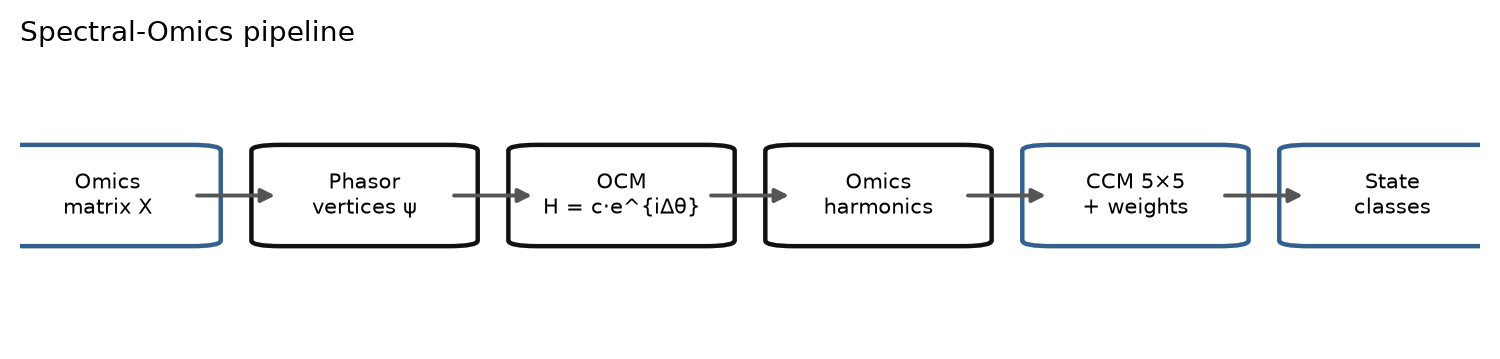
\includegraphics[width=\linewidth]{workflow.png}
\caption{\textbf{The Spectral-Omics pipeline.} An omics matrix is encoded as
phasor vertices, assembled into the Hermitian Omics Connectome Matrix,
diagonalised into omics harmonics, and read out through the $5\times5$ Omics
Stress Tensor, the Omicatome compartment weights, and the seven-class state
taxonomy; every run closes with the algebraic consistency suite.}
\label{fig:workflow}
\end{figure}

\subsection{The construction is internally consistent}
\label{sec:res-consistency}

On both datasets all seven checks of \cref{sec:theory-consistency} pass at
machine precision: Hermiticity and \OST{} Hermiticity are exact, the spectrum is
real, eigenvector orthonormality and gauge invariance hold to $\sim10^{-14}$, the
covariance form is positive semi-definite, and spectral completeness closes to
$\sim10^{-13}$. The gauge-invariance residual confirms empirically that a random
global phase shift leaves the \OCM{} spectrum unchanged, as required by
\cref{sec:theory-ocm}. These are correctness guarantees for the implementation;
the biological content is in the sections that follow.

\subsection{Tumour and normal tissue separate in spectral space}
\label{sec:res-cancer}

Running the pipeline per sample on the lung cohort (GSE10072) separates the two
tissue classes by their spectral fingerprint (\cref{fig:cancer-sep}).
Adjacent-normal tissue has low spectral entropy ($\Hspec\approx0.61$) and a large
leading gap ($\Delta_F\approx55$): its molecular network is dominated by a single
coherent collective expression mode. Tumours are spectrally \emph{fragmented} ---
higher entropy ($\Hspec\approx0.75$) and roughly half the gap
($\Delta_F\approx28$), \cref{tab:cancer} --- their expression variance spread
across many competing harmonics. This is the spectral signature of the loss of
coordinated transcriptional regulation that accompanies malignant transformation,
recovered here without supervised training and consistent with the eigengene view
that a few dominant modes capture coherent regulatory programmes
\citep{alter2000svd}.

\begin{table}[htbp]
\centering
\caption{\textbf{Spectral separation of lung tumour vs.\ normal (GSE10072).}
Per-group means; the two classes are never used during encoding or decomposition.}
\label{tab:cancer}
\small
\begin{ruledtabular}
\begin{tabular}{lccc}
Group & $n$ & spectral entropy $\Hspec$ & Fiedler gap $\Delta_F$ \\
\colrule
Normal & 49 & 0.607 & 55.4 \\
Tumour & 58 & 0.748 & 28.2 \\
\end{tabular}
\end{ruledtabular}
\end{table}

\begin{figure}[htbp]
\centering
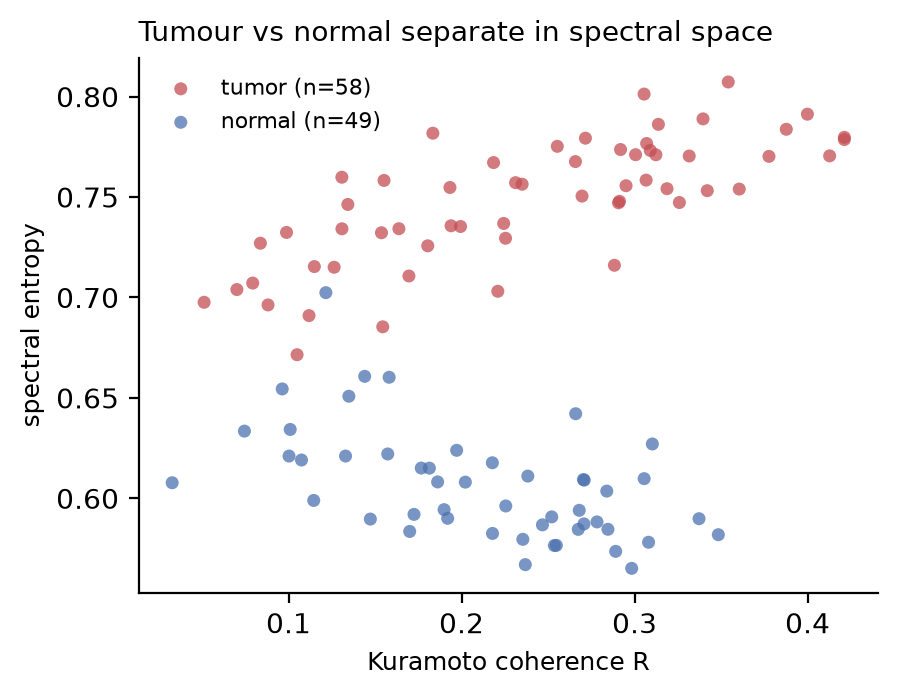
\includegraphics[width=0.82\linewidth]{cancer_indicator_separation.png}
\caption{\textbf{Spectral separation of lung tumour and normal tissue.} Each
point is one sample in the plane of Kuramoto coherence $R$ and spectral entropy
$\Hspec$ (tumour red, normal blue). The classes separate almost entirely along
$\Hspec$: normal tissue is spectrally concentrated, tumours are fragmented.}
\label{fig:cancer-sep}
\end{figure}

\begin{figure}[htbp]
\centering
\begin{subfigure}{0.49\linewidth}
  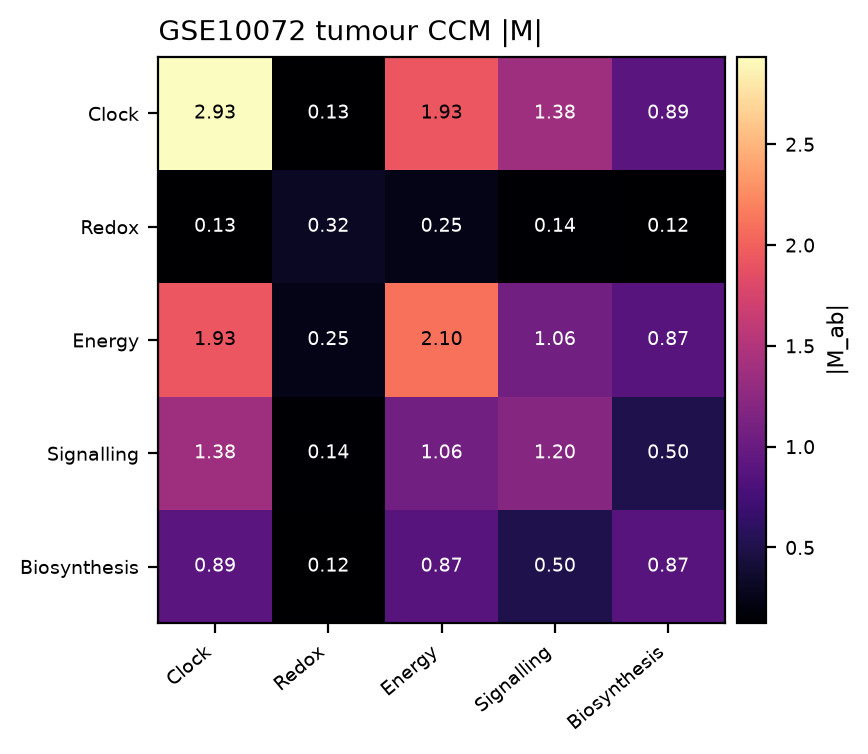
\includegraphics[width=\linewidth]{cancer_ost_heatmap.png}
  \caption{}
  \label{fig:cancer-ost}
\end{subfigure}\hfill
\begin{subfigure}{0.49\linewidth}
  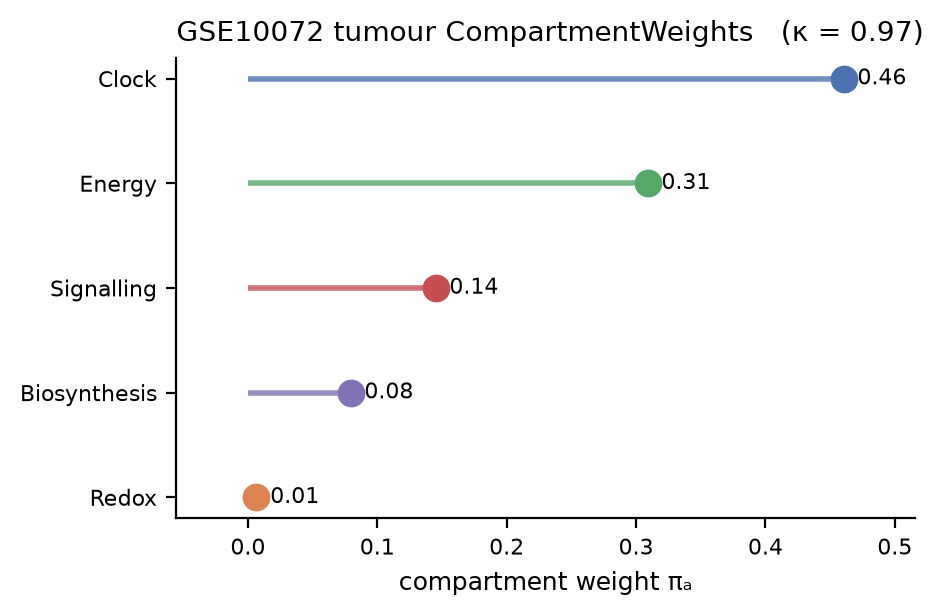
\includegraphics[width=\linewidth]{cancer_omicatome.png}
  \caption{}
  \label{fig:cancer-oma}
\end{subfigure}
\caption{\textbf{Compartment-level readout for a representative tumour.}
(a) Magnitude of the Omics Stress Tensor $|M_{ab}|$; the strong clock--energy
off-diagonal coupling reflects the tight coordination of clock and metabolism.
(b) The corresponding Omicatome compartment weights and coherence $\kappa$.}
\label{fig:cancer-ost-oma}
\end{figure}

\begin{figure}[htbp]
\centering
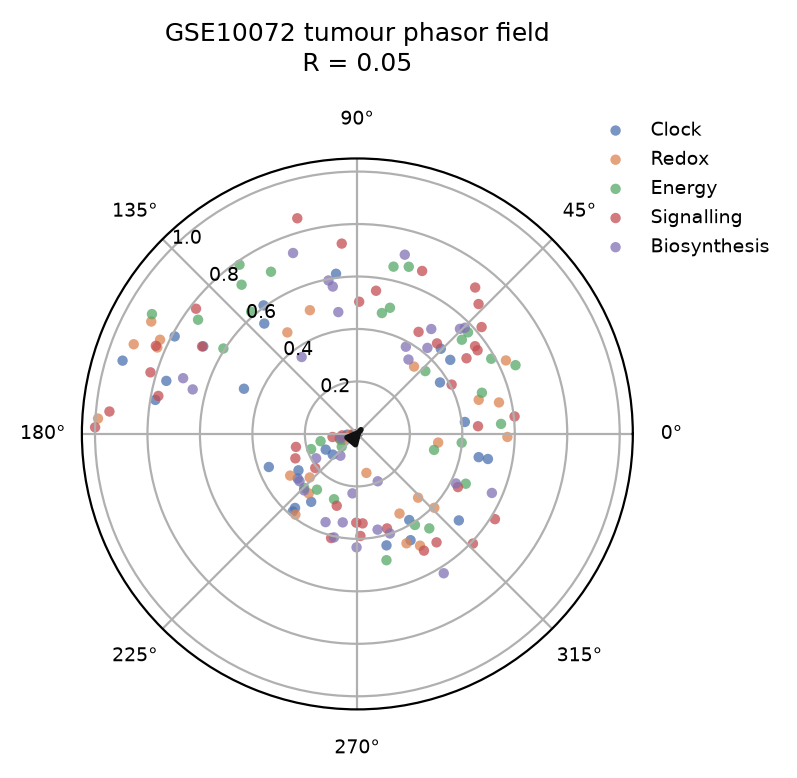
\includegraphics[width=0.62\linewidth]{cancer_phasor_snapshot.png}
\caption{\textbf{Phasor field of a lung sample.} Feature vertices are coloured by
biological compartment; the black arrow is the Kuramoto resultant
$\tfrac{1}{N}\sum_n e^{i\theta_n}$. The phase distribution is the phase-native
analog of a pathway-activity profile.}
\label{fig:cancer-phasor}
\end{figure}

\FloatBarrier

\subsection{The leading omics harmonic follows the circadian clock}
\label{sec:res-circadian}

On the mouse-liver time-course (GSE11923) the pipeline exposes a clear circadian
oscillation of the \emph{collective} spectral state. The leading eigenvalue
$\lambda_1$ traces two full $\sim$24-hour cycles across CT18--CT65 and is well fit
by a $24$-hour cosinor ($R^2 = 0.62$, acrophase near CT0, subjective dawn;
\cref{fig:circ-fit}). The oscillation is not confined to $\lambda_1$: the Fiedler
gap ($R^2 = 0.68$) and participation ratio ($R^2 = 0.66$) tighten and loosen with
the same period (\cref{fig:circ-dash}, \cref{tab:circ}), so the entire harmonic
spectrum breathes with the clock --- concentrating into a dominant mode near the
metabolic peak and dispersing at the trough. The harmonic timeline and
spectral-energy heatmap (\cref{fig:circ-timeline}) make this periodic
concentration of spectral energy directly visible, echoing the harmonic
structure of circadian transcription reported at the single-gene level
\citep{hughes2009harmonics, zhang2014circadian} but expressed here as a property
of the network's normal modes.

\begin{table}[htbp]
\centering
\caption{\textbf{$24$-hour cosinor fit of the spectral indicators (GSE11923).}
Fraction of variance $R^2$ explained by a single $24$-hour cosinor.}
\label{tab:circ}
\small
\begin{ruledtabular}
\begin{tabular}{lcccc}
 & $\lambda_1$ & $\Delta_F$ & $\PR$ & $\Hspec$ \\
\colrule
$24$-h $R^2$ & 0.62 & 0.68 & 0.66 & 0.63 \\
\end{tabular}
\end{ruledtabular}
\end{table}

\begin{figure}[htbp]
\centering
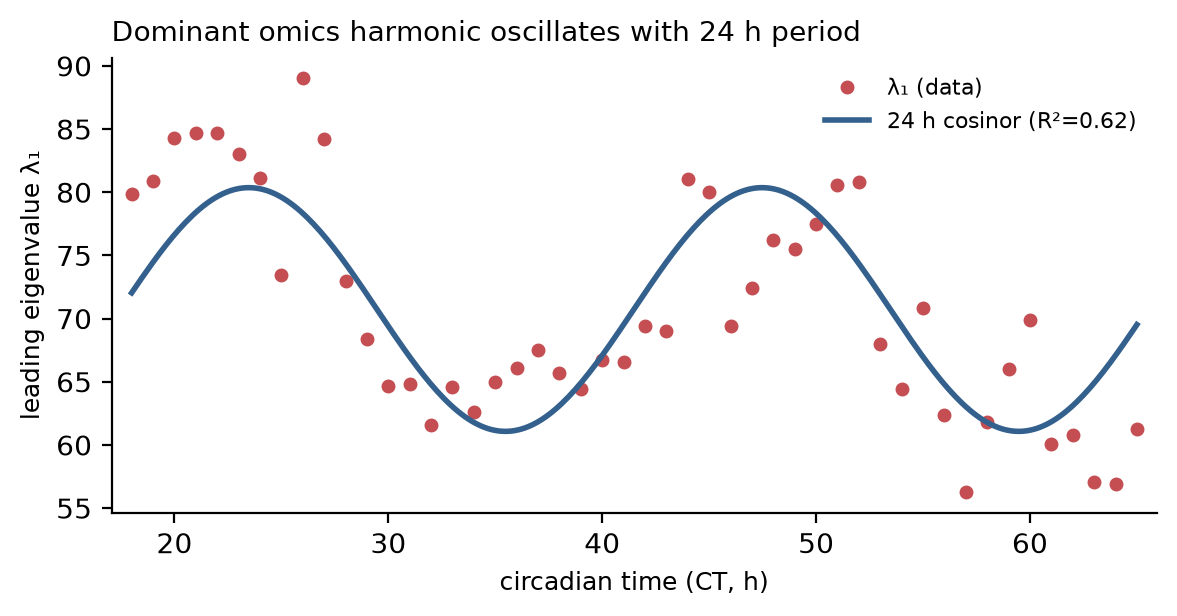
\includegraphics[width=0.9\linewidth]{circadian_leading_harmonic_fit.png}
\caption{\textbf{The leading omics harmonic oscillates with the circadian clock.}
$\lambda_1$ of the liver transcriptome (points) across CT18--CT65; the solid line
is the $24$-hour cosinor fit ($R^2 = 0.62$). Two full circadian cycles are
covered.}
\label{fig:circ-fit}
\end{figure}

\begin{figure}[htbp]
\centering
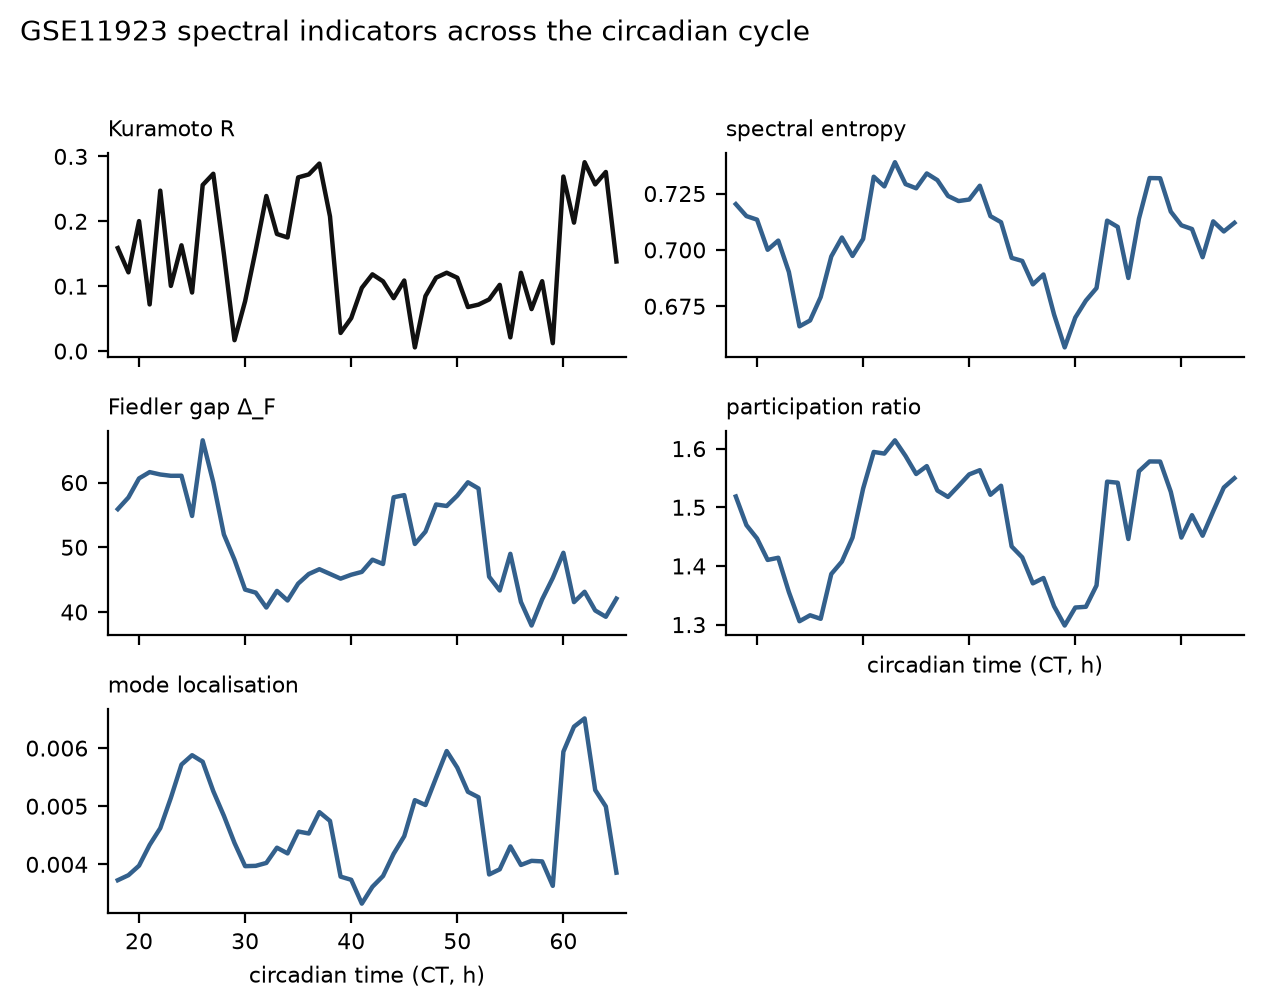
\includegraphics[width=\linewidth]{circadian_indicator_dashboard.png}
\caption{\textbf{Spectral indicators across the circadian cycle.} The Fiedler gap
and participation ratio show the strongest $24$-hour rhythm, tightening near the
metabolic peak and loosening at the trough; the algebraic connectivity, a
property of the fixed coupling alone, is omitted as it carries no per-slice
signal.}
\label{fig:circ-dash}
\end{figure}

\begin{figure}[htbp]
\centering
\begin{subfigure}{0.49\linewidth}
  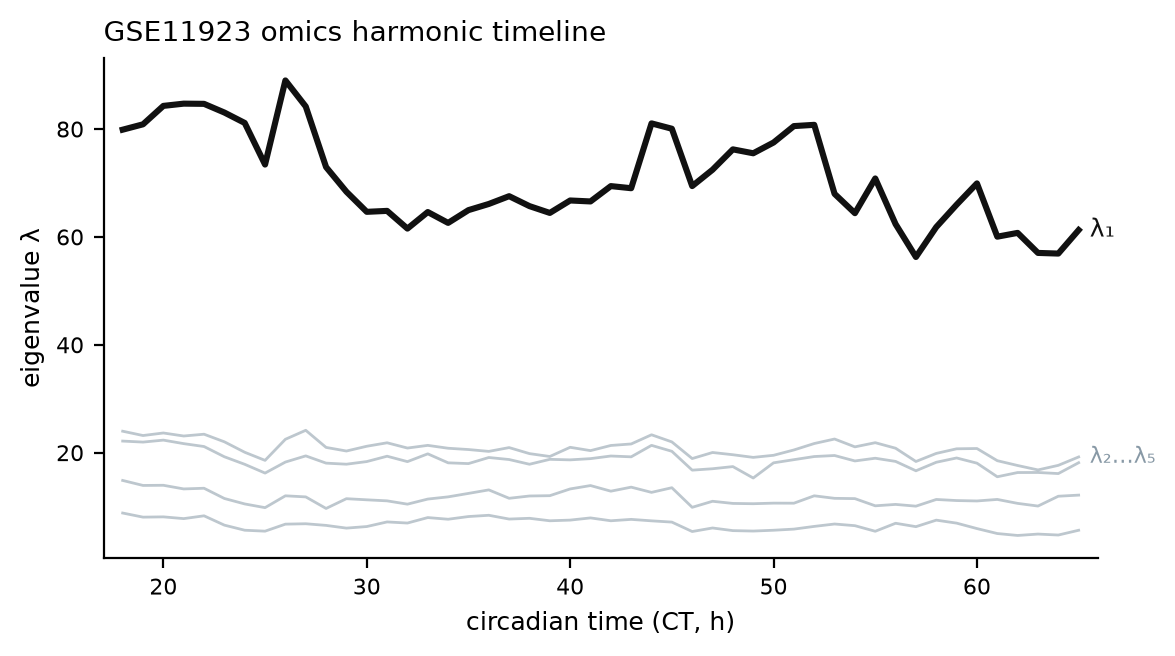
\includegraphics[width=\linewidth]{circadian_harmonic_timeline.png}
  \caption{}
  \label{fig:circ-tl}
\end{subfigure}\hfill
\begin{subfigure}{0.49\linewidth}
  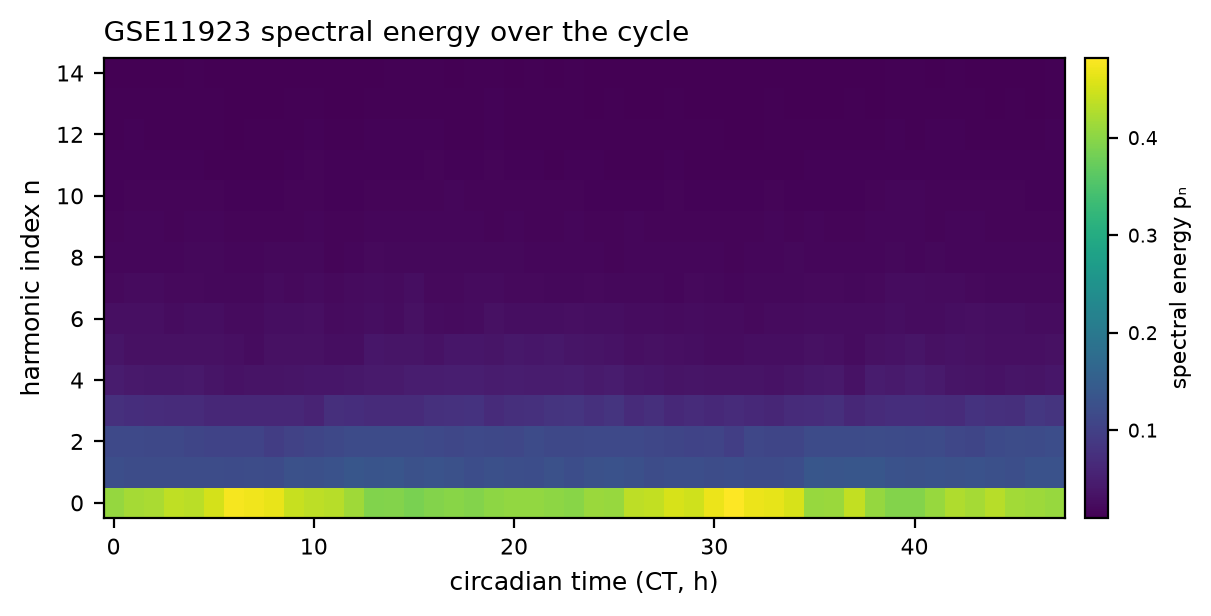
\includegraphics[width=\linewidth]{circadian_eigenvalue_heatmap.png}
  \caption{}
  \label{fig:circ-heat}
\end{subfigure}
\caption{\textbf{Time-resolved omics harmonics over the circadian cycle.}
(a) Trajectories of the leading harmonics. (b) Normalised spectral energy
$p_n(t)$; the periodic concentration into the leading modes is the spectral
signature of the clock.}
\label{fig:circ-timeline}
\end{figure}

\subsection{Phasor field and state trajectory}
\label{sec:res-phasor}

A phasor snapshot at CT18 (\cref{fig:circ-phasor}) shows feature vertices
coloured by compartment with the Kuramoto resultant overlaid; the compartments
occupy distinct phase sectors, the phase-native counterpart of a
pathway-activity profile. Across the cycle the state taxonomy of
\cref{tab:taxonomy} traces a repeating trajectory rather than resting in a single
class (\cref{fig:circ-tax}), consistent with a system driven periodically through
its regime space rather than relaxing to one fixed point.

\begin{figure}[htbp]
\centering
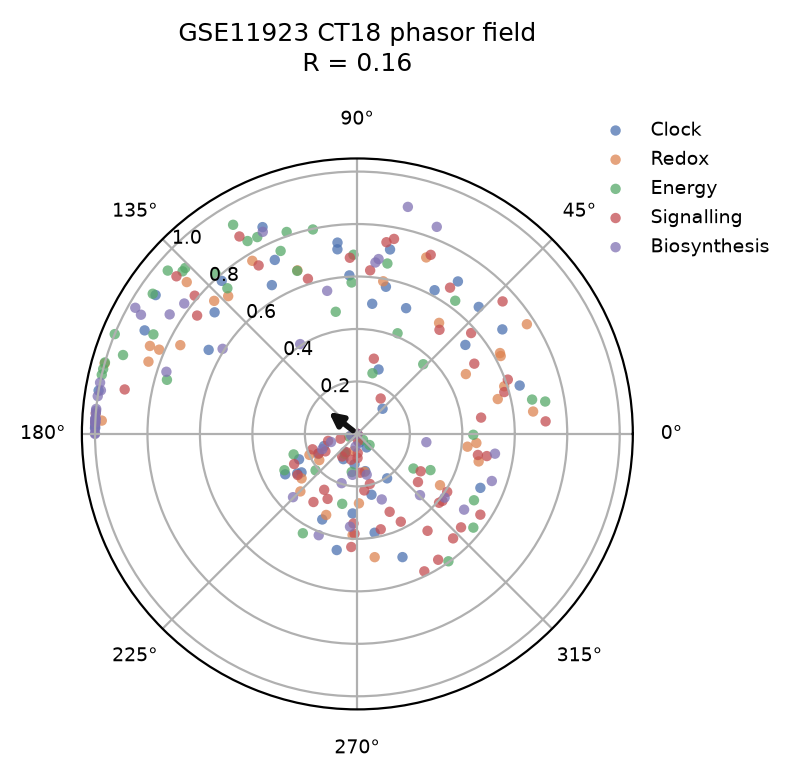
\includegraphics[width=0.62\linewidth]{circadian_phasor_snapshot.png}
\caption{\textbf{Phasor field of the liver transcriptome at CT18.} Vertices are
coloured by biological compartment; the black arrow is the Kuramoto resultant.
Compartments occupy distinct phase sectors.}
\label{fig:circ-phasor}
\end{figure}

\begin{figure}[htbp]
\centering
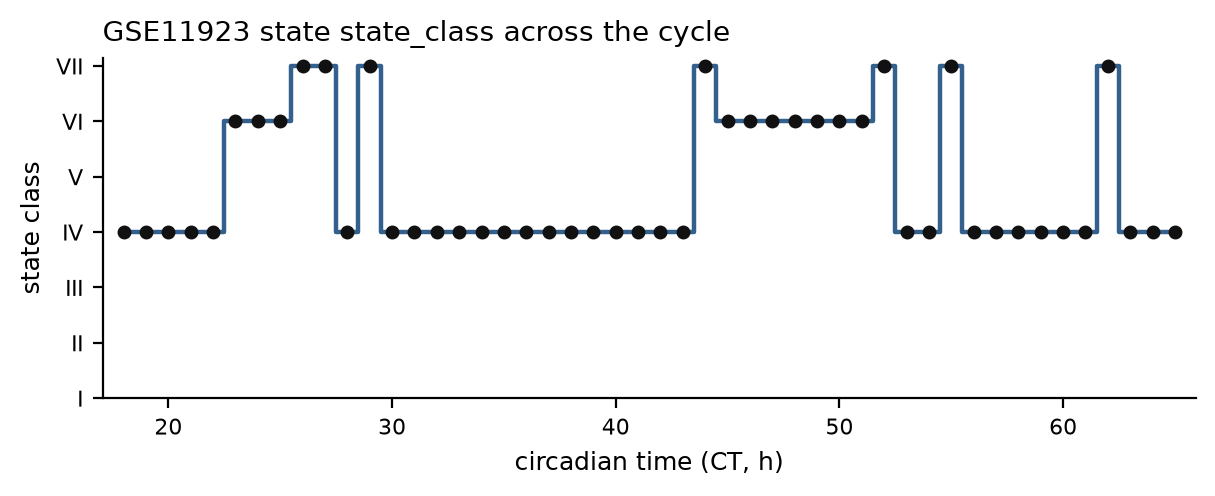
\includegraphics[width=0.9\linewidth]{circadian_taxonomy_history.png}
\caption{\textbf{State-taxonomy trajectory across the circadian cycle.} The
liver transcriptome cycles among taxonomy classes with the $\sim24$-hour period
rather than resting in one class, consistent with periodic driving.}
\label{fig:circ-tax}
\end{figure}

\FloatBarrier

% ================================================================
\section{Discussion and Conclusion}
\label{sec:conclusion}

We have presented Spectral-Omics, a phase-native graph-spectral framework for
multi-omics data. Encoding molecular features as phasor vertices and building the
amplitude-weighted Hermitian Omics Connectome Matrix turns an omics matrix into a
set of real-valued collective harmonics whose spectrum is sample-specific,
gauge-invariant, and internally consistent to machine precision. The framework
recovers biologically coherent structure on two public datasets without
supervised training: lung tumours are distinguished from normal tissue by a
fragmented spectrum, and the leading omics harmonic of the liver transcriptome
oscillates with the circadian clock.

\paragraph{Why phase helps.}
The circadian result is the clearest illustration of what the phasor encoding
adds. A magnitude-only embedding sees the liver transcriptome as a cloud of
correlated genes; the phasor \OCM{} sees a network whose \emph{collective} mode
tightens and loosens once per day. That rhythm lives in the relative phases of
the features --- precisely the degree of freedom a real-valued decomposition such
as SVD/PCA \citep{alter2000svd} cannot represent. Gauge invariance is what makes
this well posed: absolute phase is unobservable (there is no privileged zero of
the circadian cycle), and only the phase differences that survive the gauge enter
the spectrum. In this respect Spectral-Omics is to gene-expression graphs what
the phasor representation is to fluorescence decays \citep{digman2008phasor,
stringari2011cell}: a change of coordinates that makes timing and mixture
geometric.

\paragraph{Relation to existing spectral methods.}
The pipeline sits alongside a large body of spectral analysis in biology --- SVD
eigengenes \citep{alter2000svd}, co-expression modules
\citep{langfelder2008wgcna}, spectral clustering and modularity
\citep{vonluxburg2007tutorial, newman2006modularity}, connectome harmonics
\citep{atasoy2016connectome}, and diffusion maps \citep{haghverdi2015diffusion}
--- and differs from all of them in one respect: the operator being
diagonalised is Hermitian \emph{because} of a phase, so its eigenvectors encode
relative timing rather than only covariance. The $5\times5$ Omics Stress Tensor
and the Omicatome then compress the harmonics onto five named compartments,
exchanging resolution for a fixed, physiologically interpretable readout that is
directly comparable across samples.

\paragraph{Limitations and outlook.}
The present analysis uses bulk microarray data and a single global coupling; a
condition-specific or rolling coupling would let the harmonics track network
rewiring, not only phasor motion. Single-cell and spatial assays are the natural
next substrate, where the phasor field becomes a function of cell or location and
the \OST{} becomes a spatial map, and where diffusion-geometry methods are
already established \citep{haghverdi2015diffusion}. Prior-adjacency couplings from
curated regulatory or protein-interaction networks \citep{barabasi2011network}
would sharpen the compartment structure, and the curated marker list --- a
compact seed rather than an exhaustive pathway database --- is a clear target for
extension. Finally, the exact gate correspondence of \cref{sec:theory-quantum}
invites executing the spectral step on quantum hardware for networks beyond
classical diagonalisation. Spectral-Omics shows that the phase of a molecular
measurement, usually discarded, carries recoverable and biologically coherent
signal.

\section*{Code and data availability}
The \texttt{spectralomics} package, experiment scripts, and unit tests are
released with this work. Both datasets (GSE10072, GSE11923) are public and
downloaded automatically from the NCBI Gene Expression Omnibus
\citep{edgar2002geo} by the experiment scripts.

\section*{Acknowledgements}
We thank the maintainers of the public data repositories whose datasets made
this study possible.

\bibliographystyle{apsrev4-2}
\bibliography{references}

\end{document}
